\documentclass[]{article}
\usepackage{lmodern}
\usepackage{amssymb,amsmath}
\usepackage{ifxetex,ifluatex}
\usepackage{fixltx2e} % provides \textsubscript
\ifnum 0\ifxetex 1\fi\ifluatex 1\fi=0 % if pdftex
  \usepackage[T1]{fontenc}
  \usepackage[utf8]{inputenc}
\else % if luatex or xelatex
  \ifxetex
    \usepackage{mathspec}
  \else
    \usepackage{fontspec}
  \fi
  \defaultfontfeatures{Ligatures=TeX,Scale=MatchLowercase}
\fi
% use upquote if available, for straight quotes in verbatim environments
\IfFileExists{upquote.sty}{\usepackage{upquote}}{}
% use microtype if available
\IfFileExists{microtype.sty}{%
\usepackage{microtype}
\UseMicrotypeSet[protrusion]{basicmath} % disable protrusion for tt fonts
}{}
\usepackage[margin=1in]{geometry}
\usepackage{hyperref}
\hypersetup{unicode=true,
            pdftitle={auto-insurance},
            pdfauthor={Krista Waugh},
            pdfborder={0 0 0},
            breaklinks=true}
\urlstyle{same}  % don't use monospace font for urls
\usepackage{color}
\usepackage{fancyvrb}
\newcommand{\VerbBar}{|}
\newcommand{\VERB}{\Verb[commandchars=\\\{\}]}
\DefineVerbatimEnvironment{Highlighting}{Verbatim}{commandchars=\\\{\}}
% Add ',fontsize=\small' for more characters per line
\usepackage{framed}
\definecolor{shadecolor}{RGB}{248,248,248}
\newenvironment{Shaded}{\begin{snugshade}}{\end{snugshade}}
\newcommand{\KeywordTok}[1]{\textcolor[rgb]{0.13,0.29,0.53}{\textbf{#1}}}
\newcommand{\DataTypeTok}[1]{\textcolor[rgb]{0.13,0.29,0.53}{#1}}
\newcommand{\DecValTok}[1]{\textcolor[rgb]{0.00,0.00,0.81}{#1}}
\newcommand{\BaseNTok}[1]{\textcolor[rgb]{0.00,0.00,0.81}{#1}}
\newcommand{\FloatTok}[1]{\textcolor[rgb]{0.00,0.00,0.81}{#1}}
\newcommand{\ConstantTok}[1]{\textcolor[rgb]{0.00,0.00,0.00}{#1}}
\newcommand{\CharTok}[1]{\textcolor[rgb]{0.31,0.60,0.02}{#1}}
\newcommand{\SpecialCharTok}[1]{\textcolor[rgb]{0.00,0.00,0.00}{#1}}
\newcommand{\StringTok}[1]{\textcolor[rgb]{0.31,0.60,0.02}{#1}}
\newcommand{\VerbatimStringTok}[1]{\textcolor[rgb]{0.31,0.60,0.02}{#1}}
\newcommand{\SpecialStringTok}[1]{\textcolor[rgb]{0.31,0.60,0.02}{#1}}
\newcommand{\ImportTok}[1]{#1}
\newcommand{\CommentTok}[1]{\textcolor[rgb]{0.56,0.35,0.01}{\textit{#1}}}
\newcommand{\DocumentationTok}[1]{\textcolor[rgb]{0.56,0.35,0.01}{\textbf{\textit{#1}}}}
\newcommand{\AnnotationTok}[1]{\textcolor[rgb]{0.56,0.35,0.01}{\textbf{\textit{#1}}}}
\newcommand{\CommentVarTok}[1]{\textcolor[rgb]{0.56,0.35,0.01}{\textbf{\textit{#1}}}}
\newcommand{\OtherTok}[1]{\textcolor[rgb]{0.56,0.35,0.01}{#1}}
\newcommand{\FunctionTok}[1]{\textcolor[rgb]{0.00,0.00,0.00}{#1}}
\newcommand{\VariableTok}[1]{\textcolor[rgb]{0.00,0.00,0.00}{#1}}
\newcommand{\ControlFlowTok}[1]{\textcolor[rgb]{0.13,0.29,0.53}{\textbf{#1}}}
\newcommand{\OperatorTok}[1]{\textcolor[rgb]{0.81,0.36,0.00}{\textbf{#1}}}
\newcommand{\BuiltInTok}[1]{#1}
\newcommand{\ExtensionTok}[1]{#1}
\newcommand{\PreprocessorTok}[1]{\textcolor[rgb]{0.56,0.35,0.01}{\textit{#1}}}
\newcommand{\AttributeTok}[1]{\textcolor[rgb]{0.77,0.63,0.00}{#1}}
\newcommand{\RegionMarkerTok}[1]{#1}
\newcommand{\InformationTok}[1]{\textcolor[rgb]{0.56,0.35,0.01}{\textbf{\textit{#1}}}}
\newcommand{\WarningTok}[1]{\textcolor[rgb]{0.56,0.35,0.01}{\textbf{\textit{#1}}}}
\newcommand{\AlertTok}[1]{\textcolor[rgb]{0.94,0.16,0.16}{#1}}
\newcommand{\ErrorTok}[1]{\textcolor[rgb]{0.64,0.00,0.00}{\textbf{#1}}}
\newcommand{\NormalTok}[1]{#1}
\usepackage{graphicx,grffile}
\makeatletter
\def\maxwidth{\ifdim\Gin@nat@width>\linewidth\linewidth\else\Gin@nat@width\fi}
\def\maxheight{\ifdim\Gin@nat@height>\textheight\textheight\else\Gin@nat@height\fi}
\makeatother
% Scale images if necessary, so that they will not overflow the page
% margins by default, and it is still possible to overwrite the defaults
% using explicit options in \includegraphics[width, height, ...]{}
\setkeys{Gin}{width=\maxwidth,height=\maxheight,keepaspectratio}
\IfFileExists{parskip.sty}{%
\usepackage{parskip}
}{% else
\setlength{\parindent}{0pt}
\setlength{\parskip}{6pt plus 2pt minus 1pt}
}
\setlength{\emergencystretch}{3em}  % prevent overfull lines
\providecommand{\tightlist}{%
  \setlength{\itemsep}{0pt}\setlength{\parskip}{0pt}}
\setcounter{secnumdepth}{0}
% Redefines (sub)paragraphs to behave more like sections
\ifx\paragraph\undefined\else
\let\oldparagraph\paragraph
\renewcommand{\paragraph}[1]{\oldparagraph{#1}\mbox{}}
\fi
\ifx\subparagraph\undefined\else
\let\oldsubparagraph\subparagraph
\renewcommand{\subparagraph}[1]{\oldsubparagraph{#1}\mbox{}}
\fi

%%% Use protect on footnotes to avoid problems with footnotes in titles
\let\rmarkdownfootnote\footnote%
\def\footnote{\protect\rmarkdownfootnote}

%%% Change title format to be more compact
\usepackage{titling}

% Create subtitle command for use in maketitle
\newcommand{\subtitle}[1]{
  \posttitle{
    \begin{center}\large#1\end{center}
    }
}

\setlength{\droptitle}{-2em}

  \title{auto-insurance}
    \pretitle{\vspace{\droptitle}\centering\huge}
  \posttitle{\par}
    \author{Krista Waugh}
    \preauthor{\centering\large\emph}
  \postauthor{\par}
      \predate{\centering\large\emph}
  \postdate{\par}
    \date{3/7/2019}


\begin{document}
\maketitle

\begin{Shaded}
\begin{Highlighting}[]
\KeywordTok{library}\NormalTok{(readr)}
\KeywordTok{library}\NormalTok{(ggplot2)}
\KeywordTok{library}\NormalTok{(dplyr)}
\end{Highlighting}
\end{Shaded}

\begin{verbatim}
## 
## Attaching package: 'dplyr'
\end{verbatim}

\begin{verbatim}
## The following objects are masked from 'package:stats':
## 
##     filter, lag
\end{verbatim}

\begin{verbatim}
## The following objects are masked from 'package:base':
## 
##     intersect, setdiff, setequal, union
\end{verbatim}

\begin{Shaded}
\begin{Highlighting}[]
\KeywordTok{library}\NormalTok{(tidyverse)}
\end{Highlighting}
\end{Shaded}

\begin{verbatim}
## -- Attaching packages ----------------------------------------------------------------------------------------------------------------- tidyverse 1.2.1 --
\end{verbatim}

\begin{verbatim}
## √ tibble  1.4.2     √ purrr   0.2.5
## √ tidyr   0.8.1     √ stringr 1.3.1
## √ tibble  1.4.2     √ forcats 0.3.0
\end{verbatim}

\begin{verbatim}
## -- Conflicts -------------------------------------------------------------------------------------------------------------------- tidyverse_conflicts() --
## x dplyr::filter() masks stats::filter()
## x dplyr::lag()    masks stats::lag()
\end{verbatim}

\begin{Shaded}
\begin{Highlighting}[]
\NormalTok{data <-}\StringTok{ }\KeywordTok{read_csv}\NormalTok{(}\StringTok{"decal_midterm.csv"}\NormalTok{)}
\end{Highlighting}
\end{Shaded}

\begin{verbatim}
## Parsed with column specification:
## cols(
##   `Claim Number` = col_double(),
##   AGE = col_double(),
##   INCOME = col_character(),
##   MARITAL_STATUS = col_character(),
##   EDUCATION = col_character(),
##   MVR_POINTS = col_double(),
##   CAR_AGE = col_double(),
##   LOCATION = col_character(),
##   OLD_CLAIM = col_character(),
##   PREMIUM = col_character()
## )
\end{verbatim}

\begin{Shaded}
\begin{Highlighting}[]
\KeywordTok{colnames}\NormalTok{(data) =}\StringTok{ }\KeywordTok{c}\NormalTok{(}\StringTok{"claim_number"}\NormalTok{, }\StringTok{"age"}\NormalTok{, }\StringTok{"income"}\NormalTok{, }\StringTok{"marital_status"}\NormalTok{, }\StringTok{"education"}\NormalTok{, }\StringTok{"mvr_points"}\NormalTok{, }\StringTok{"car_age"}\NormalTok{, }\StringTok{"location"}\NormalTok{, }\StringTok{"old_claim"}\NormalTok{, }\StringTok{"premium"}\NormalTok{)}
\NormalTok{data}
\end{Highlighting}
\end{Shaded}

\begin{verbatim}
## # A tibble: 8,161 x 10
##    claim_number   age income marital_status education mvr_points car_age
##           <dbl> <dbl> <chr>  <chr>          <chr>          <dbl>   <dbl>
##  1            1    60 $67,3~ No             PhD                3      18
##  2            2    43 $91,4~ No             High Sch~          0       1
##  3            3    35 $16,0~ Yes            High Sch~          3      10
##  4            4    51 $64,6~ Yes            <High Sc~          0       6
##  5            5    50 $114,~ Yes            PhD                3      17
##  6            6    34 $125,~ No             Bachelors          0       7
##  7            7    54 $18,7~ Yes            <High Sc~          0       1
##  8            8    37 $107,~ Yes            Bachelors         10       7
##  9            9    34 $62,9~ No             Bachelors          0       1
## 10           10    50 $106,~ No             Bachelors          1      17
## # ... with 8,151 more rows, and 3 more variables: location <chr>,
## #   old_claim <chr>, premium <chr>
\end{verbatim}

\begin{Shaded}
\begin{Highlighting}[]
\NormalTok{age <-}\StringTok{ }\KeywordTok{select}\NormalTok{(data, age, mvr_points)}
\NormalTok{age}
\end{Highlighting}
\end{Shaded}

\begin{verbatim}
## # A tibble: 8,161 x 2
##      age mvr_points
##    <dbl>      <dbl>
##  1    60          3
##  2    43          0
##  3    35          3
##  4    51          0
##  5    50          3
##  6    34          0
##  7    54          0
##  8    37         10
##  9    34          0
## 10    50          1
## # ... with 8,151 more rows
\end{verbatim}

\begin{Shaded}
\begin{Highlighting}[]
\KeywordTok{ggplot}\NormalTok{(age, }\KeywordTok{aes}\NormalTok{(age, mvr_points)) }\OperatorTok{+}\StringTok{ }\KeywordTok{geom_point}\NormalTok{()}
\end{Highlighting}
\end{Shaded}

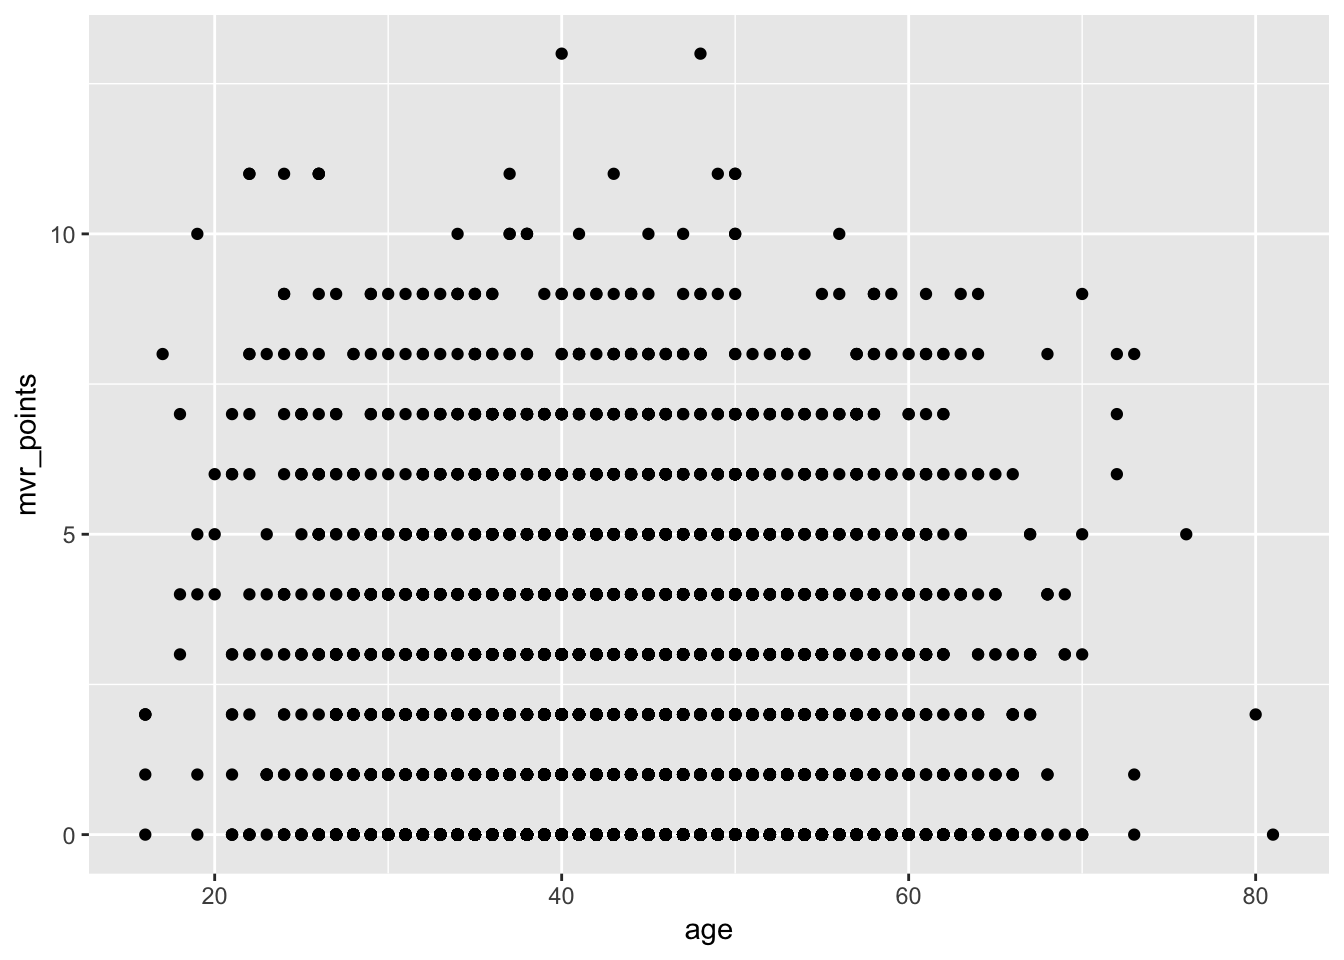
\includegraphics{auto-insurance_files/figure-latex/unnamed-chunk-3-1.pdf}

\begin{Shaded}
\begin{Highlighting}[]
\NormalTok{income <-}\StringTok{ }\KeywordTok{select}\NormalTok{(data, income, mvr_points)}

\KeywordTok{ggplot}\NormalTok{(income, }\KeywordTok{aes}\NormalTok{(income, mvr_points)) }\OperatorTok{+}\StringTok{ }\KeywordTok{geom_point}\NormalTok{(}\DataTypeTok{size =}\NormalTok{ .}\DecValTok{5}\NormalTok{)}
\end{Highlighting}
\end{Shaded}

\includegraphics{auto-insurance_files/figure-latex/unnamed-chunk-4-1.pdf}

\begin{Shaded}
\begin{Highlighting}[]
\NormalTok{marital_status <-}\StringTok{ }\KeywordTok{select}\NormalTok{(data, marital_status, mvr_points)}

\KeywordTok{ggplot}\NormalTok{(marital_status, }\KeywordTok{aes}\NormalTok{(marital_status, mvr_points)) }\OperatorTok{+}\StringTok{ }\KeywordTok{geom_col}\NormalTok{(}\DataTypeTok{binwidth =} \DecValTok{2}\NormalTok{)}
\end{Highlighting}
\end{Shaded}

\begin{verbatim}
## Warning: Ignoring unknown parameters: binwidth
\end{verbatim}

\includegraphics{auto-insurance_files/figure-latex/unnamed-chunk-5-1.pdf}

\begin{Shaded}
\begin{Highlighting}[]
\NormalTok{phd <-}\StringTok{ }\KeywordTok{filter}\NormalTok{(data, education }\OperatorTok{==}\StringTok{ "PhD"}\NormalTok{)}
\NormalTok{highschool <-}\StringTok{ }\KeywordTok{filter}\NormalTok{(data, education }\OperatorTok{==}\StringTok{ "High School"}\NormalTok{)}
\NormalTok{bachelor  <-}\StringTok{ }\KeywordTok{filter}\NormalTok{(data, education }\OperatorTok{==}\StringTok{ "Bachelors"}\NormalTok{)}
\NormalTok{under_highschool <-}\StringTok{ }\KeywordTok{filter}\NormalTok{(data, education }\OperatorTok{==}\StringTok{ "<High School"}\NormalTok{)}
\end{Highlighting}
\end{Shaded}

\begin{Shaded}
\begin{Highlighting}[]
\NormalTok{education <-}\StringTok{ }
\StringTok{  }\KeywordTok{ggplot}\NormalTok{(, }\KeywordTok{aes}\NormalTok{(}\DataTypeTok{y =}\NormalTok{ data}\OperatorTok{$}\NormalTok{mvr_points)) }\OperatorTok{+}
\StringTok{  }\KeywordTok{geom_col}\NormalTok{(}\DataTypeTok{x =}\NormalTok{ phd) }\OperatorTok{+}
\StringTok{  }\KeywordTok{geom_col}\NormalTok{(}\DataTypeTok{x =}\NormalTok{ bachelor) }\OperatorTok{+}
\StringTok{  }\KeywordTok{geom_col}\NormalTok{(}\DataTypeTok{x =}\NormalTok{ highschool) }\OperatorTok{+}
\StringTok{  }\KeywordTok{geom_col}\NormalTok{(}\DataTypeTok{x =}\NormalTok{ under_highschool)}
\NormalTok{education}
\end{Highlighting}
\end{Shaded}

\begin{Shaded}
\begin{Highlighting}[]
\NormalTok{car <-}\StringTok{ }\KeywordTok{select}\NormalTok{(data, car_age, mvr_points)}

\KeywordTok{ggplot}\NormalTok{(car, }\KeywordTok{aes}\NormalTok{(car_age, mvr_points)) }\OperatorTok{+}\StringTok{ }\KeywordTok{geom_jitter}\NormalTok{()}
\end{Highlighting}
\end{Shaded}

\includegraphics{auto-insurance_files/figure-latex/unnamed-chunk-8-1.pdf}

\begin{Shaded}
\begin{Highlighting}[]
\NormalTok{rural_urban <-}\StringTok{ }
\StringTok{  }\KeywordTok{select}\NormalTok{(data, )}
\end{Highlighting}
\end{Shaded}

\begin{Shaded}
\begin{Highlighting}[]
\NormalTok{phd <-}\StringTok{ }\KeywordTok{filter}\NormalTok{(data, education }\OperatorTok{==}\StringTok{ "PhD"}\NormalTok{)}
\NormalTok{highschool <-}\StringTok{ }\KeywordTok{filter}\NormalTok{(data, education }\OperatorTok{==}\StringTok{ "High School"}\NormalTok{)}
\NormalTok{bachelor  <-}\StringTok{ }\KeywordTok{filter}\NormalTok{(data, education }\OperatorTok{==}\StringTok{ "Bachelors"}\NormalTok{)}
\NormalTok{under_highschool <-}\StringTok{ }\KeywordTok{filter}\NormalTok{(data, education }\OperatorTok{==}\StringTok{ "<High School"}\NormalTok{)}
\end{Highlighting}
\end{Shaded}


\end{document}
